\chapter{State of The Art} \label{chap:sota}


% TODO chapter description
%To understand the applications and characteristics of GANs, a simple search for "Generative Adversarial Networks" was performed on Google Scholar\footnote{Google Scholar \url{https://scholar.google.com/}}. The most relevant paper was written by Goodfellow et al. \cite{goodfellow.etal_GenerativeAdversarialNets_} where they discussed the architecture of the newly developed generative adversarial network, possible improvements and some applications (refer to sec. \ref{sec:gan_background}). A brief comparison between other generative models is also performed. In the following years, Conditional GANs \cite{goodfellow.etal_GenerativeAdversarialNets_} were proposed to improve the productive performance; Wasserstein GANs \cite{arjovsky.etal_WassersteinGenerativeAdversarial_} introduced a new loss function that provides some stability during the training process; in Radford et al. \cite{radford.etal_UnsupervisedRepresentationLearning_2016} deep convolutional networks were used for both the generator and discriminator which showed a significant performance increase when generating images. Since then, many variations have emerged to tackle different problems.

%Most GANs were designed for problems with image datasets; however, the dataset used in this study consists only of tabular data. With this, the focus of the search shifted from conventional GANs for image applications to ones more focused on tabular data. During this search phase, the previously unknown area of detection of anomalies with GANs surfaced. Because of this, state of the art for this study will be divided into two parts. The first pertains to the more prevalent architectures for tabular generation, and the other focuses on GANs applied to anomaly detection on table datasets.

A Systematic Literature Review (SLR) was performed to understand the current trends of clustering methods and the use of GANs for anomaly detection. This chapter is divided into two parts. The first part will focus on the relevant clustering methods for this work. The second part will focus on the most relevant GAN architectures for anomaly detection. Each part will start with the definition of the search questions and the search queries. Next, the inclusion/exclusion criteria for the obtained results are identified. Finally, the results are presented and discussed.


The first part (sec. \ref{sec:gan_background}) will focus on the most relevant GAN architectures for anomaly detection. The second part (sec. \ref{sec:clustering_methods}) will focus on the most relevant clustering methods.


A Systematic Literature Review (SLR) was performed to understand the current trends of GANs applied to anomaly detection and clustering methods. This search method allows for the analysis of all the existing research on a defined question. To achieve this, a set of search questions is formulated (sec. \ref{sec:search_questions}) and grouped into two search queries (sec. \ref{sec:search_queries}). Next, the inclusion/exclusion criteria for the obtained results are identified (sec. \ref{sec:inclusion_exclusion}).


\section{Clustering}\label{sec:sota_clustering}
\subsection{Search Questions}\label{sec:cluster_search_questions}

\subsection{Search Query}\label{sec:cluster_search_queries}

\subsection{Inclusion/Exclusion Criteria}\label{sec:cluster_inclusion_exclusion}

\subsection{Results}\label{sec:cluster_results}
\begin{description}
    \item[Jain]\cite{Jain_Dataclustering50_2010} performs an extensive review of the K-Means algorithm. The author defines clusters as representations of $n$ objects separated into $k$ groups based on a similarity measure. The use cases for the application of clustering are also defined. These include the discovery of the underlying data structures, natural classification (degree of similarity between forms) and compression (a method for the organization and summarization of data).
    
    A brief analysis of the history of clustering is provided, where the author shows the use of clustering methods in a wide range of fields and a brief explanation of hierarchical and partition-based clustering algorithms. Next, an explanation of the base K-Means algorithm is presented along with a discussion of the parameters that need to be defined by the user. In addition, an analysis of other clustering methods, such as DBSCAN and CLIQUE is performed. 

    In the next sections, the author explains the importance of the data representation and the features chosen for the clustering task. A discussion on the decision of the correct number of clusters is also performed, to which the author concludes that there is no definitive answer.

    The next section explains the concept of cluster validity, which evaluates the results of cluster analysis in a quantitive and objective manner. The validity criteria assess the internal cluster structure, the degree of separation between structures and the degree of correspondence between the clustering and the external information (class labels). Possible cluster admissibility criteria are also presented. These are defined by rules that aim to ensure that clusters do not intersect each other and that the chosen algorithm provides the same results on data with different transformations, such as scaling.
    
    Finally, the authors enumerate a set of guidelines that should be taken into account when choosing a clustering algorithm, based on the criteria discussed in the previous sections.
\end{description}

% \begin{description}
%     \item[ConsensusClusterPlus] \cite{Wilkerson.Hayes_ConsensusClusterPlusclassdiscovery_2010} is an unsupervised class discovery method, used in cancer research to discover intrinsic groups sharing the same biological characteristics. The goal of the authors was to determine how many groups were in a dataset and to determine their number with confidence.
    
%     The implementation is based on the preexisting consensus clustering method, which is a resampling-based approach that assesses the stability of clusters. The authors extended this method by allowing the use of new clustering algorithms and improving the visualization techniques used to infer the number of classes.

%     % TODO rever
% \end{description}

\begin{description}
    \item[Rodriguez et al.]\cite{Rodriguez.Laio_Clusteringfastsearch_2014} propose that cluster centers have a higher density than their neighbors and are at a higher distance from other cluster centers. In addition, the proposed algorithm is resilient to outliers as it identified them and excludes them from the analysis. 
    
    The proposed method is capable of detecting non-spherical clusters and identifying the correct number of clusters, like DBSCAN. Cluster centers are determined by selecting the points with the local maxima density values. The algorithm works by calculating the density of each point in the dataset and the distance from that point to other high-density points. After this step, the other points that are not considered centers are assigned to the nearest high-density point. This is done in a single step, making this algorithm more efficient than previous ones. 

    To evaluate the implementation, tests are conducted on synthetic point distributions and compared with other clustering algorithms. The results show that the algorithm is capable of reliantly detecting cluster structures in the different datasets. The authors also conclude that the algorithm is robust to changes in the scale of the dataset (as long as it doesn't affect the distances of the points) and that the approach is more practical than other methods, as it does not require the definition of parameters such as the probability distribution.
\end{description}

\begin{description}
    \item[Fahad et al.]\cite{Fahad.Alshatri.ea_SurveyClusteringAlgorithms_2014a} provide a detailed analysis of the application of different classes of clustering methods on big data. The goal of the authors is to overcome the shortcomings of other surveys by systematically categorizing clustering algorithms; presenting the advantages and disadvantages of each class of algorithms; providing several evaluation measures; and finally analyzing the most representative algorithm of each category.
    
    The authors identify five different clustering algorithm categories. These are partitioning, hierarchical, density-based, grid-based and model-based. A set of clustering algorithms is identified for each of the categories.

    In the next section, the authors categorize the clustering methods in accordance with three properties of big data. These are volume, velocity and variety. The first refers to the ability of the algorithm to deal with large datasets with high dimensionality and also includes the existence of outliers. Velocity refers to the time complexity of the algorithms. And finally, variety refers to the ability of the algorithm to deal with different types of data, and the cluster shapes that are produced by it.

    The choice of algorithm for each of the categories is done by picking the ones that satisfy most of the above-defined criteria. An explanation of the algorithm is provided for each of the candidates. In the testing phase, eight simulated datasets, ranging from denial of service (DOS) attacks to water treatment operation logs, were used. Each of the candidates is evaluated based on the validity of the generated clusters, the stability\footnote{Some clustering algorithms are based on a random component, which can lead to varying results in different executions.} of the algorithms and the total execution time. The results show that no algorithm is capable of satisfying all the criteria and that the choice of the algorithm depends on the type of data and the desired results.
\end{description}

\begin{description}
    \item[Kou et al.]\cite{Kou20141} intend to evaluate several clustering algorithms on financial risk datasets as a multiple criteria decision-making problem (MCDM). The reason for this methodology is the lack of objective measures to determine the quality of clustering algorithms. The authors propose validating clusters in terms of external and internal assessment and a relative test. Internal criteria evaluate the similarity of observations inside a cluster, while external measure the inter-cluster distances. Relative tests take advantage of previous knowledge of the dataset, such as class labels.
    
    The process of clustering algorithm evaluation is divided into four steps. The first step is to select three financial risk datasets. Next, six popular clustering algorithms are picked to perform clustering on each of the datasets. In the third step, the authors aggregate eleven performance metrics into a single matrix for each of the datasets. Finally, the resulting matrices are passed through three MCDM methods that rank the clustering methods for each of the datasets.

    The results showed that the K-Means repeated bisection algorithm was the overall best choice for the chosen financial risk datasets, despite some disagreements between the MCDM methods. The authors conclude that more research efforts should be undertaken to find compromised solutions when MCDM methods disagree.
\end{description}


\begin{description}
    \item[CAN]\cite{Nie.Wang.ea_Clusteringprojectedclustering_2014a} (Clustering with Adaptive Neighbors) is a clustering algorithm that can simultaneously learns data similarity matrix and clustering structure. Its goal is to assign the adaptive and optimal neighbors of each point in the dataset. For this, the authors assume that data points with smaller distances should have larger probabilities of being neighbors. In addition, the algorithm imposes a constraint on the Laplacian of the similarity matrix so that the number of connected components in the data is the same as the number of clusters.
    
    Projected Clustering with Adaptive Neighbors (PCAN) for high-dimensionality data is also implemented and is used to attenuate the difficulties in performing clustering on datasets with many features. The main goal of this was to reduce the dimension of the data without hindering the goals of the developed adaptive neighbors' algorithm.

    In the experimentation phase, the authors start by testing the CAN algorithm in a toy dataset consisting of two clusters, in which the algorithm can detect reliably both connected components. Next, a comparison is performed with K-Means on a synthetic clustering dataset, in which CAN outperforms the other method in terms of accuracy. PCAN is tested alongside, two other dimensionality reduction methods, PCA and Locality Preserving Projections (LPP). The projection, as well as the clustering abilities, are evaluated for each of the reduction methods. PCAN can find the correct subspaces for the projection task in contrast with the other methods. In addition, the clustering results after the projection are also more reliable than the other methods. 

    Finally, CAN and PCAN alongside other clustering methods are tested with real-world datasets. The results showed that both methods outperformed the other baselines in every dataset (but one) in terms of accuracy. CAN and PCAN alternated in the different datasets with one outperforming the other in each of them.
\end{description}

\begin{description}
    \item[Granato et al.]\cite{Granato.Santos.ea_Useprincipalcomponent_2018} provide a critical analysis on the use of principal Component Analysis (PCA) and Hierarchical Clustering Algorithms (HCA) in the field of bioactive compounds. In this field, the discipline of chemometrics\footnote{Science of extracting information from chemical processes using mathematics and statistics information.} is often used to assess the differences/similarities between observations or to project them into lower dimensions. 
    
    First, the authors provide a brief explanation of PCA is presented followed by an example of its application on fruit juices' chemical composition and antioxidant activity. The number of components that explain the most variance is decided by analyzing the cumulative explained variance of the dataset of PCAs with different numbers of components. The results showed that 81\% of the data variation was explained by two components, with the first explaining 50\% and the other 31\%. After this example, an state-of-the-art analysis is provided on the use of PCA in food science studies.

    In the next section, a brief explanation of HCA and the approaches to resolving the grouping problem is provided.  The agglomerative approach considers every data point as a cluster in the beginning of the algorithm and then merges the cluster in pairs. The second method, divisive, starts with a single cluster and then divides it into smaller ones. In addition, the most used metrics of sample distance and linkage methods are enumerated. As in the previous section, an analysis of the state-of-the-art of application of HCA in food science is done. 
    
    In the end, the authors provide an example to explain the most common problem faced with the use of PCA and HCA in this field. They start by applying PCA to project the data samples into two dimensions. An analysis of the results showed that in one of the classes, the existence of outliers made it so some of the samples were significantly further away than the others. Then by applying HCA, it was demonstrated that different linkage distances produced varying numbers of clusters and that these would ultimately need to be decided be the user. With this simple example, they conclude that HCA and PCA should be avoided in this field and that the calculation of correlation coefficients would, in most cases, provide a better analysis of the data at hand.
\end{description}

\begin{description}
    \item[Lin et al.]\cite{Lin.Tsai.ea_Clusteringbasedundersamplingclassimbalanced_2017}  propose a clustering-based undersampling method for class-imbalanced datasets. The authors propose overcoming the shortcomings of undersampling methods, which come with the risk of excluding important features from the majority class. To achieve this, they intend to replace the random undersampling strategy with clustering methods. By using undersampling to cluster the majority class will yield clusters with a similar size to the minority class. 
    
    An analysis of the traditional methods for resampling and classifier ensembles is first introduced. These include methods such as synthetic minority oversampling (SMOTE), random undersampling (RUS) and Underbagging (UB). Next, the main hypothesis of the work is presented in the form of clustering-based undersampling. The process consists of first dividing an imbalanced dataset, $D$, into training and test sets. In the second step, the training data is divided into majority and minority class sets. In the following phase, the clustering-based undersampling method is used to reduce the number of samples in the majority class. Finally, the balanced training set is used to train a classifier, which is then used to classify the test set. 

    The authors present two strategies for clustering-based undersampling. In the first, the number of clusters is equal to the number of observations in the minority class. Then KMeans is applied to the majority class, $M$, producing k cluster centers (centroids), which are then used to replace the entire majority class data. In the end, the number of observations will be the same for both the majority and minority classes. In the second strategy, the same method is used to cluster the majority class. However, instead of using cluster centroids to reduce a single cluster into one observation, the authors fetch the sample in the cluster which is closest to the centroid (in terms of Euclidean distance). Both samples produce the same number of clusters, but the results from the latter are slightly different from the former.

    Two studies were conducted to evaluate both of the methods discussed in the previous section. The first to evaluate the performance of the methods in several small datasets and the other in two large datasets. Five classifiers were used to examine the classification performance, along with five state-of-the-art resampling methods. For the first study, results showed that the proposed methods significantly outperformed the baseline in terms of the receiver operator characteristic (ROC) curve. In addition, the nearest neighbor clustering-based undersampling method scored higher than the centroid-based one. The best classifier, in terms of accuracy (from the initial five), was the multilayer perceptron (MLP). In the second, study, the results were mostly the same, with the best classifer (C4.5) being better than the MLP from the previous test.

    The authors conclude that the design ensembles are well suited as a substitute for the traditional resampling methods and discuss the possibility of employing feature and instance selection to filter out unrepresentative features and data samples. In addition, other state-of-the-art classification algorithms could be combined with the clustering-based undersampling method to try and yield better results.
\end{description}


\begin{description}
    \item[Douzas et al.]\cite{Douzas.Bacao.ea_Improvingimbalancedlearning_2018} developed a novel heuristic oversampling method based on KMeans and SMOTE. The main goal is to overcome the common issues of SMOTE, such as the overfitting of the training data and the generation of noisy samples. Clustering allows for the oversampler to target areas of input where the generation of artificial data is safer by ignoring noisy regions. 
    
    The algorithm is divided into three parts: clustering, filtering and oversampling. In the first step the input is clustered into k clusters. Then, during the filtering phase, the clusters that have higher proportions of minority class samples are retained. In the final step, SMOTE is applied to each of the selected clusters to achieve the desired target ratio of minority and majority instances. 

    The effectiveness of the algorithm is compared with three classifiers trained on several imbalanced datasets for binary classification problems. Each dataset was subjected to five other oversampling techniques and then used to train the classification models. A model with unaltered data was also trained for each of the datasets. The results showed that models trained with the K-Means SMOTE method outperformed not only the ones trained on the original data but also the models trained with data after the application of the baseline oversampling methods.
\end{description}

\begin{description}
    \item[K-Shape]\cite{Paparrizos.Gravano_kShapeEfficientAccurate_2015a} is a highly accurate and efficient clustering algorithm for time-series data. In this paper, the authors propose a scale/translate/shift-invariant distance measure derived from a cross-correlation measure; present a new way of calculating cluster centroids with the new distance measure; and develop a new algorithm for time-series data based on the previous two.
    
    An enumeration and explanation of five possible time-series invariances is provided. These include scaling and translation invariances, shift, uniform scaling, occlusion and complexity invariances. The authors conclude that some of these problems, like scale and translation invariances, can be attenuated by normalizing the input data beforehand. However, the less straightforward ones can be resolved by choosing a proper distance metric. Following this, the Euclidean Distance and Dynamic Time Warping (DTW) metrics are point out as the most prevalent distance measures for time-series data. Further details are provided for the state-of-the-art clustering algorithms and time-series averaging techniques, after which the hypothesis is formulated. In it, the authors set out to solve the scaling and shifting invariance problems.

    The method is based on the calculation of time-series centroids with the cross-correlation metric. This measure captures the shape of similar signals by ignoring the shifts in phase and amplitude, making it possible to determine the similarity of two sequences even if they are not aligned. In addition, it is concluded that a normalization of the input data is necessary to achieve the best possible comparisons. After this, a new shape-based distance measure (SBD) is formulated around the cross-correlation statistic and data normalization techniques.

    In the following sections, a detailed explanation of the algorithm is provided based on the application of the newly defined distance measure and possible optimizations. The algorithm starts by randomly assigning time-series sequences to clusters and then computes the centroids of each cluster with the \textit{ShapeExtraction} algorithm based on the SBD distance measure. Finally, the algorithm refines the memberships of the clusters with the help of the same distance algorithm. This process is repeated up to 100 times or until the centroids do not change (convergence).

    In the testing phase, the authors compare the SBD measure with the Euclidean Distance and two variations of the DTW measure. Six clustering baselines are selected to compare with the developed algorithm. At the end of the experiments, it was concluded that cross-correlation measures are as competitive as other distance metrics such as DTW, but are significantly faster. The authors note that the choice of clustering method is as important as the distance measure and that the K-Means with Euclidean distance is the clustering method for time-series data. However, K-Shape outperformed every other state-of-the-art and was significantly faster than K-Means with Euclidean distance.
\end{description}

\begin{description}
    \item[DPC-KNN]\cite{Du.Ding.ea_Studydensitypeaks_2016} is a density peak-based clustering algorithm developed to overcome the shortcomings of the original density peaks clustering (DPC) algorithm \cite{Rodriguez.Laio_Clusteringfastsearch_2014}, which is not capable of detecting clusters with different densities. The authors propose a new method for determining the density of each point based on the KNN algorithm. 
    
    In addition to the main problem regarding the density of the clusters, the authors also identify other issues with the original algorithm. These include the difficulty in handling high dimensional data which tends to confuse DPC by hiding clusters in noisy data; and the inability of the algorithm to take into account local geometries of clusters. 
    
    To solve this last issue, the authors propose changing the way the density of each point is calculated. In the original algorithm, the density of a point is calculated as the distance between that point and every other point in the data. In the new method, the density of a point is calculated as the mean distance between that point and its k nearest neighbors. This change allows the algorithm to take into account the local geometry of the clusters. The dimensionality problem is solved by applying PCA, on the previous DPC-KNN, resulting in the DPC-KNN-PCA method.

    In the testing phase, the authors perform experiments on several 2D synthetic datasets, in which DPC-KNN achieved perfect scores. In the next experiments, real-life datasets with high dimensionality are used to test the effectiveness of both DPC-KNN methods with DPC and the other baselines. In the end, the authors conclude that DPC-KNN outperforms every other method in terms of accuracy in low-dimensionality data, with data with more than seven features resulting in better results for DPC-KNN-PCA.
\end{description}





\section{Adversarial Anomaly Detection}\label{sec:sota_anomaly_detection}

\subsection{Search Questions}\label{sec:gan_search_questions}
Two search questions were defined to find out the most relevant articles that would more closely fit the needs of this work:

%\noindent\textbf{SQ1} \textit{What are the current GAN architectures for anomaly detection?} GANs are a pervasive field of research with many different applications. For this work, we are only interested in the subset that pertains to the use of GANs for anomaly detection.

\noindent\textbf{SQ1} \textit{What are the current GAN-based architectures for anomaly detection in tabular data?} Most GANs are designed for problems with image datasets. However, the dataset used in this study consists only of tabular data. The intent is to include only GANs designed or adapted to anomaly detection in tabular datasets.

\noindent\textbf{SQ2} Of the results from the previous question, which ones can generate new samples following the distribution of the dataset and detect out-of-distribution examples? The proposed goals for this thesis are to produce a model that can generate new solar wind profiles and another that can accurately distinguish out-of-distribution samples from normal ones. As so, the generator should be able to generate examples in the same distribution as the original dataset, while the discriminator must distinguish anomalous ones.

\subsection{Search Query}\label{sec:gan_search_queries}
The search questions defined in the previous sections were aggregated into a single search query. The query construction was incremental to narrow the search results to the desired questions. In the end, the search query was the following:
\begin{center}
\textbf{(gan*  OR  adversarial learning  OR  generative adversarial net*) \\ AND (( anomal*  OR  outlier?  OR  abnormal  OR  novel* )  AND  detect* ) \\ AND NOT  (imag*  OR  video*  OR  segment* OR photo*)}
\end{center}

The first part consists of a mixture of terms associated with GANs and intendeds to only retrieve articles with one of those terms in the title, abstract and keywords. The second restricts the results to GANs for outlier detection in the same three fields as the previous one. Several synonyms for outlier were used to increase the number of relevant papers. The final term was only applied to the documents' keywords and was intended to exclude GANs applied to image datasets. All articles were retrieved from Scopus \footnote{Scopus: \url{https://www.scopus.com/}}.

%As previously stated, to achieve the goals of this study, we are interested in mainly two search topics. The first consists of GAN architectures designed/adapted to handle tabular data and was performed on Google Scholar\footnote{Google Scholar \url{https://scholar.google.com/}}. For this, a combination of related terms and abbreviations for "generative adversarial networks" and "tabular data" was used (1000 results at the end). The second search topic, which can be considered a subtopic of the first, pertains to the use of GANs for anomaly detection in table datasets and is performed on Scopus\footnote{Scopus: \url{https://www.scopus.com/}}. The same identifying terms for GANs were used, but with a combination of synonyms for outliers (e.g., "anomaly", "novelty", and "abnormal") to redirect the search for the area of anomaly detection (yielded 1400 results).

\subsection{Inclusion and exclusion criteria}\label{sec:gan_inclusion_exclusion}
The query defined in the previous section yielded 1489 results, making the analysis of each one by hand prohibitive. A set of criteria was determined to reduce the number of documents that needed to be studied (see Table \ref{tab:criteria}). Note that E3 only exists because the search question SQ2 failed in instances where the documents did not indicate the use of images in the keywords. These were later used with several steps to exclude non-relevant papers and narrow the state-of-the-art analysis iteratively. 

\begin{table}[ht]
\caption{Inclusion and Exclusion criteria.}
\label{tab:criteria}
\begin{tabularx}{\textwidth}{@{}llX@{}}
\hline
\textbf{Criteria}                                       & \textbf{ID} & \textbf{Description}                                                                                                                                     \\ \midrule
\multirow{4}{*}{Inclusion}                     & I1 & The document focuses on GANs for anomaly detection.                                                                                             \\
                                               & I2 & The results are clear, and the proposed goals are achieved.                                                                                     \\
                                               & I3 & The authors provide code or an extensive explanation of the architecture.                                                                       \\
                                               & I4 & Provides a comparison of the developed GAN with other baseline models (not necessarily GANs).                                                   \\ \midrule
\multicolumn{1}{c}{\multirow{4}{*}{Exclusion}} & E1 & The article was cited less than 6 times. For earlier publications, the number of citations was reduced to half.                                 \\
\multicolumn{1}{c}{}                           & E2 & Surveys and reports on works carried out by other authors.                                                                                      \\
\multicolumn{1}{c}{}                           & E3 & Does not use tabular data. Either it has one or more unwanted terms in the title (e.g. image "photo") or only performs tests on image datasets. \\
\multicolumn{1}{c}{}                           & E4 & Was published before 2014. \\\hline                                                                                                                    
\end{tabularx}
\end{table}

An illustration of the processing pipeline can be seen in Fig. \ref{fig:slr_pipeline}. 1489 results were retrieved from Scopus with the defined query. The first processing setup applies exclusion criteria \textit{E1} to remove papers with little to no citations, which resulted in 168 documents. 61 were left after a preliminary title analysis with the criteria (I1; E2-E3). In the final step, a preliminary analysis of the remaining documents' abstracts and conclusions was undertaken to only select the most relevant to the defined search questions. The inclusion criteria for this step were I1 to I4. In addition, the documents that were surveys or reviews of multiple implementations and articles that did not deal with tabular data were excluded. In the next section, the resulting papers from this last step will be explained.

\begin{figure}[htp]
\centering
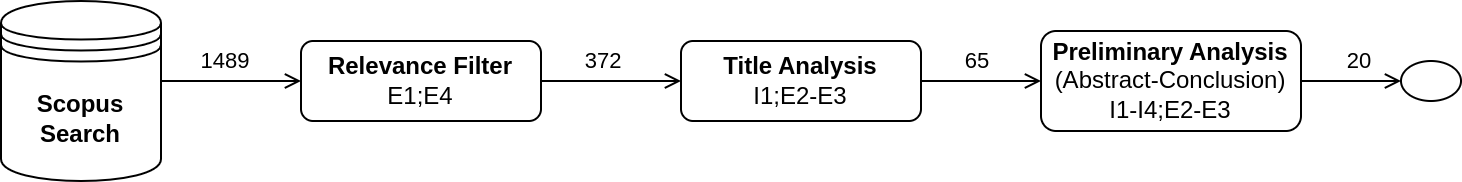
\includegraphics[width=\textwidth]{figures/slr_pipeline.png}
\caption{Systematic Literature Review Pipeline}
\label{fig:slr_pipeline}
\end{figure}




\subsection{Results}\label{sec:gan_sota_results}

\begin{description}
    \item[MAD-GAN \cite{li.etal_MADGANMultivariateAnomaly_2019}] is an architecture intended for anomaly detection in multivariate data with spatio-temporal correlations. The generator and the discriminator are composed of Long-Short-Term Recurrent Neural Networks (LSTM-RNN). As is usual in other GANs, the generator creates fake samples from a vector of latent points and feeds them to the generator, whose goal is to distinguish generated from original samples. However, instead of just using the discriminator to detect abnormal samples in the testing phase, the authors propose employing the generator for the same task. The theory for this is that by generating correct samples, the generator can learn the normal distribution of the dataset. 
    
    During the test phase, the discriminator receives a sample from the test dataset and performs the same classification as in the previous stage. However, the generator will receive a version of the sample mapped to the latent space and be tasked with reconstructing the sample. Next, the reconstruction error is calculated by comparing the reconstructed sample with the original one. This error and the discriminator outputs are used to compute the \textit{Discriminator and Reconstruction Anomaly Score} (DR-Score). A sample is considered abnormal if it has a DR-Score higher than a predefined value $\tau$. 
    
    The developed architecture was compared with five baselines. These include PCA, K-Nearest Neighbours (KNN), Feature Bagging (FB), an Autoeconder (AE), and the \textit{Efficient GAN} (EGAN) \cite{zenati.etal_EfficientGANBasedAnomaly_2018a}. The tests were performed on three intrusion detection datasets. MAD-GAN was able to outperform the other baselines on almost all datasets consistently.
\end{description}

\begin{figure}[htp]
\centering
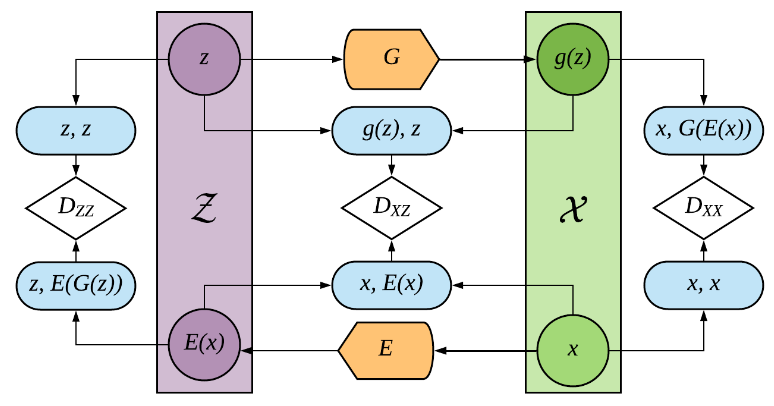
\includegraphics[width=0.8\textwidth]{figures/alad_architecture.png}
\caption[ALAD Architecture]{ALAD Architecture. $D_{xx}$, $D_{xz}$ and $D_{xx}$ are the discriminators (white), $Z$ (purple) and $X$ (green) represent the latent and data spaces, respectively; $G$ and $E$ (orange) are the generator and the encoder, respectively. Reprinted from \cite{zenati.etal_AdversariallyLearnedAnomaly_2018}.}
\label{fig:alad_arch}
\end{figure}

\begin{description}
    \item[ALAD \cite{zenati.etal_AdversariallyLearnedAnomaly_2018}] is a reconstruction-based anomaly detection architecture that employs multiple bi-directional GANs. The proposed method, \textit{Adversarily Learned Anomaly Detection} (ALAD), intends to use both the discriminator and the generator for the task. The ALAD architecture can be seen in Fig. \ref{fig:alad_arch}.
    
    An encoder network $E$ maps data samples $x$ into the latent space $z$ during training. Several additional discriminators are used to achieve cycle consistency (to ensure that the reconstructed samples resemble the original ones) and to provide stability to the model. $D_{xz}$ is an improvement from other similar solutions that solve the saddle-point problem by ensuring cycle consistency, which is not always the case when using encoders. Further entropy regularisation is imposed on both $G$ and $E$ by the discriminators $D_{xx}$ and $D_{zz}$. The latter receives two pairs of latent points and must distinguish the real ($z$, $z$) from the synthesized one ($z$, $E(x)$); the former follows a similar logic but with examples extracted from the dataset. 
    
    The authors propose a new score function for anomaly detection that captures the confidence of $D_{xx}$ when distinguishing real from synthesized pairs. This is because a poor-quality reconstruction would indicate that the generator did not learn how to reconstruct that sample and, consequently, should be considered an anomaly. Finally, the designed model was compared with five standard anomaly detection methods and another GAN for anomaly detection on two anomaly detection datasets. The developed model outperformed the baselines on one of the datasets but could not do so on the other. This was because this dataset had a small number of samples, and ALAD, like other GANs, requires large amounts of training data.
\end{description}

\begin{description}
    \item[USAD \cite{audibert.etal_USADUnSupervisedAnomaly_2020}] is an architecture based on adversarially trained autoencoders for anomaly detection in multivariate time series data, more concretely, logs from IT systems. The authors proposed solving the convergence and mode collapse problems experienced in other GANs. USAD is composed of one encoder $E$ and two decoders $D1$ and $D2$, which in conjunction with the encoder, result in two autoencoders ($AE1$ and $AE2$). $E$ takes data samples as windows $W$ and encodes them to latent space vectors $z$. The function of the decoders is to reconstruct the samples in those windows. 
    
    The autoencoders are trained with normal samples to learn the data distribution during this phase. In the detection stage, both autoencoders are trained adversarially. $AE1$ reconstructs samples from the real dataset and $AE2$ must distinguish examples reconstructed by $AE1$ from the real data. The anomaly score is calculated based on the reconstruction errors obtained on both autoencoders. The proposed model was evaluated along with other unsupervised methods for anomaly detection on intrusion detection datasets. USAD outperformed the other baselines in terms of F1-Score.
\end{description}

\begin{figure}[htp]
\centering
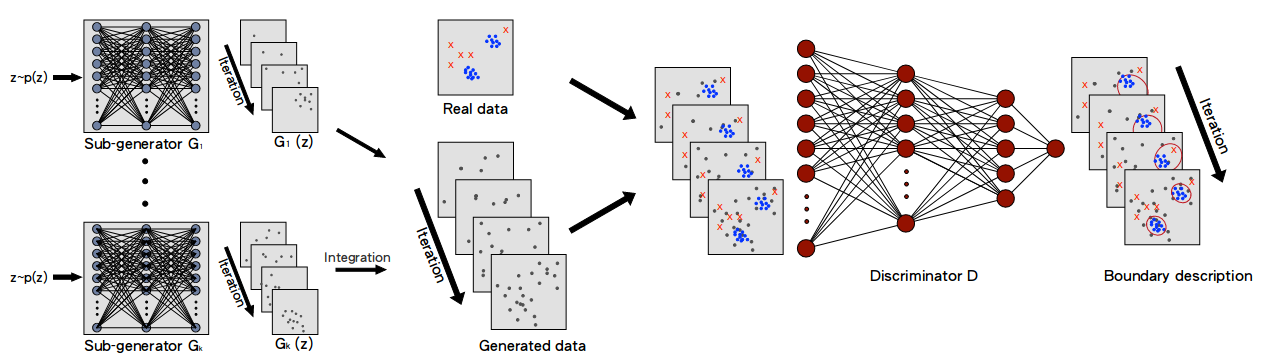
\includegraphics[width=\textwidth]{figures/moogal_arch.png}
\caption[MO-GAAL Architecture]{MO-GAAL Architecture. Each generator $G_i$ to $G_k$ (left) generates outliers for the respective cluster; The discriminator $D$ (right) aims to draw increasingly smaller boundaries around the real data distribution. Taken from \cite{liu.etal_GenerativeAdversarialActive_2020}.}
\label{fig:mo_gaal_arch}
\end{figure}

\begin{description}
    \item[MO-GAAL \cite{liu.etal_GenerativeAdversarialActive_2020}] as the goal of generating informative outliers to overcome the significant class imbalance and lack of correct labels in outlier detection datasets. The authors developed two proximity-based outlier detection methods that do not rely on previous knowledge of the dataset. The first one was given the name of \textit{Single-objective Generative Adversarial Active Learning} (SO-GAAL). Like other GANs, it plays the same mini-max game between the generator $G$ and the discriminator $D$. However, the objective for $G$ is to produce outliers that occur inside or close to the real data. Similarly, the goal of $D$ is to create a division boundary that separates the real data from potential outliers. $G$ gradually learns the generating mechanism and synthesizes an increasing number of potential outliers, and $D$ gets better at creating the divisions that enclose the real data. The point of generating outliers is to create a reasonable reference distribution for the real data. 
    
    Despite providing good results, the first model proved to be very unstable due to the problem of mode collapse. At some point, after a good amount of iterations, the precision of the model would greatly diminish. To solve this issue, another technique called \textit{Multiple-objective Generative Active Learning} (MO-GAAL) was designed. A general workflow of the architecture can be seen in Fig. \ref{fig:mo_gaal_arch}. The authors proposed generating outliers for specific real data subsets using a generator for each cluster in the dataset (which requires cluster identification). This solved the mode collapse problem on the first model and stabilized the performance.  
    
    Both architectures were tested on fourteen datasets and ten other baseline outlier detection methods. Despite other methods performing better in specific datasets, MO-GAAL proved to be more reliable even on non-cluster datasets.
\end{description}

\begin{figure}[htp]
\centering
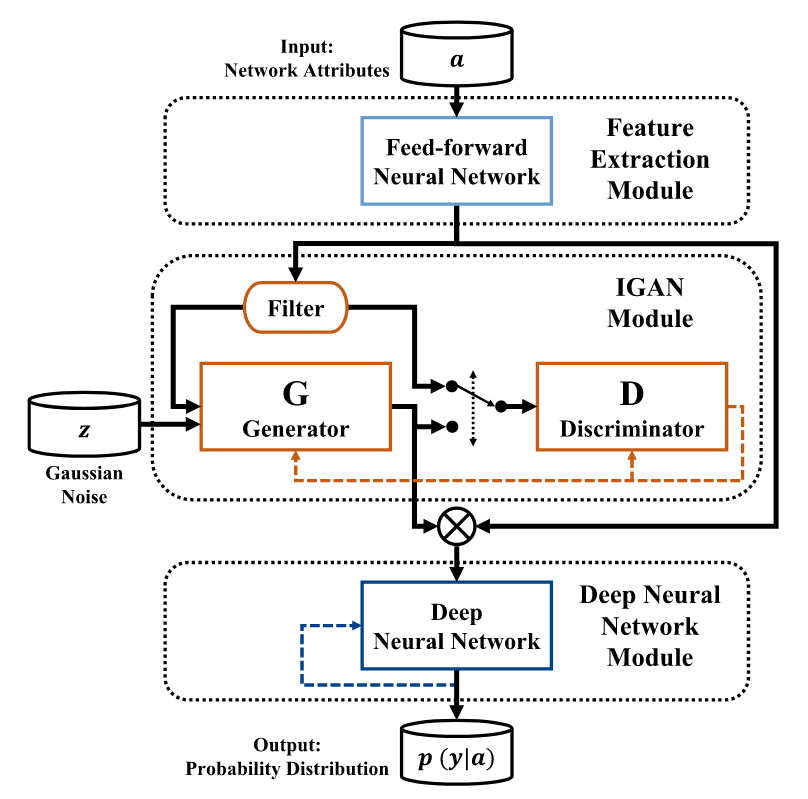
\includegraphics[scale=0.5]{figures/igan_ids_arch.png}
\caption[IGAN-IDS Architecture]{Full IGAN-IDS architecture. Taken from \cite{huang.etal_IGAN_2020}.}
\label{fig:igan_ids}
\end{figure}


\begin{description}
    \item[IGAN-IDS \cite{huang.etal_IGAN_2020}] or \textit{Imbalanced Generative Network} was designed to cope with class imbalance problems that other outlier methods for intrusion detection suffer from. IGAN, which can be seen in Fig. \ref{fig:igan_ids} (middle module) is composed of an imbalanced data filter, Generator $G$, and a Discriminator $D$. Each sample, $s=(x,y)$, is a vector containing the values and the class labels. The imbalanced filter takes only samples from the minority classes, denoted as $s'=(x', y')$. It calculates the generating factor $k$ for each class (ratio of samples that should be generated for each minority class).  $G$ receives a set of latent points $z$ and the class label $y'$ and outputs a vector with a generated value $G(z,y')$ from the class label that it received. This vector is then passed to the discriminator, which aims to distinguish synthesized feature vectors from the ones extracted from the dataset. In the training process, $G$ and $D$ are trained alternatively. First, $D$ is fed only real samples while $G$ is fixed, and in the next iteration, $G$ is optimized, and $D$ is fixed. 
    
    With the problem of class imbalance dealt with, the authors set out to perform intrusion detection with IGAN-IDS (Fig. \ref{fig:igan_ids}). The feature extraction module (top) embeds discrete data into one-hot encoded vectors and discretizes continuous variables, which are encoded. All values are concatenated and fed to IGAN, which generates samples for the imbalanced classes. Finally, a DNN (bottom module) is used for outlier detection. In the training stage, it receives both synthesized and real data and, during the testing phase, calculates the distributed probabilities for each inclusion class of each sample. The proposed solution was tested with several other class-balancing techniques on three standard intrusion detection datasets. It outperformed every method in precision, accuracy, recall and AUC score.
\end{description}


\begin{description}
    \item[Jiang et al. (2019) \cite{jiang.etal_GANBasedAnomalyDetection_2019}] propose a conditional GAN architecture to detect anomalies in univariate Industrial Time Series Data. The model is trained with only normal samples. The dimensionality of the original data was reduced by employing a feature extractor. The generator consists of two encoders $G_e$ and $G_{e'}$ and an intermediate decoder $G_d$. The first encoder maps real samples into the latent space $z$ while the decoder $G_d$ is tasked with reconstructing the encoded sample back to the real data space. 
    
    During training, the GAN is only tasked with reconstructing normal data samples so that both components learn the normal distribution of the dataset. Two loss functions are defined for the generator, the \textit{Apparent loss} and the \textit{Latent loss}. The first measures the distance between the original and synthesized samples, and the other measures the distance between the latent vectors $z$ and $z´$ encoded by $G_e$ and $G_{e'}$, respectively. The loss function of the discriminator compares the feature vector from the actual sample $f(x)$ with the synthesized one $f(G(x))$. The anomaly score is defined as the sum of the two losses. 

In the testing phase, two rolling bearing datasets were used. The authors fine-tunned the models by adjusting the hyper-parameters of the network. A significant difference in anomaly score $A(x)$ was observed for faulty parts in the dataset, which proved the efficacy of the designed model. A comparison was also performed with the state-of-the-art BiGAN \cite{donahue.etal_AdversarialFeatureLearning_2017}, which showed that the developed GAN was more reliable on datasets with differing sizes.
\end{description}

\begin{description}
    \item[TadGAN \cite{geiger.etal_TadGANTimeSeries_2020}] aims to solve the problem of scalability and portability in state-of-the-art unsupervised methods for anomaly detection. Its goal is to detect anomalies in time series datasets. The authors used LSMT Recurrent Neural networks for both the generator and the critic. Two types of anomalies are identified single point (abnormal data point) and collective (sequence of abnormal data points) anomalies. 
    
    The proposed architecture is a reconstruction-based anomaly detector with a generator $G$ which receives encoded samples in the form of latent points $z$ and reconstructs them back to the original sample distribution; an encoder that takes samples in the normal distribution and encodes them into latent point vectors; and two critics, one to distinguish real data points from synthesized ones ($C_x$) and the other ($C_z$) to evaluate between the distribution of real $z$ and the ones that were encoded by $E$ ($E(x)$). To cope with the mode collapse problem, common in most GANs, the authors adopt the Wasserstein loss function (for critics) and a cycle consistency loss function (for the generator and encoder). For the reconstruction errors, the point-wise difference (distance between the real and synthesized point)  and area difference (distance between "windows" of the same area in the real and synthesized data) were defined. Furthermore, the authors also chose a \textit{Dynamic Time Warp} (DTW) measure, which, similarly to area difference, can identify minor differences over long periods but can also handle time shift issues. 
    
    Two methods of combining the critic outputs with the reconstruction errors were devised. For the first, a weighted sum of the reconstruction error and the critic output is done; in the other method, both values are directly multiplied. Several baselines are chosen to compare with the developed model in the testing phase. TadGAN and the baselines were tested on eleven datasets for anomaly detection (two of which were from NASA). The developed network outperformed every other baseline on six of the eleven datasets (based on the F1-score). Despite this, the mean, standard deviation and average of the F1-score in all datasets showed that TadGAN was more reliable than the other methods. Finally, the authors defined ten iterations of TadGAN, each with a different anomaly score with either one reconstruction function, one critic output or a combination of the two. The worst result was with the anomaly function consisting only of the critic output, and the best was the one in which the critic score and DTW were multiplied.
\end{description}

\begin{description}
    \item[adVAE \cite{wang.etal_AdVAESelfadversarialVariational_2020}] employs a Variational Autoencoder (VAE) for anomaly detection. The authors propose an encoder $E$ that encodes real samples into random point vectors $z$, fed to a generator $G$ that is then tasked with synthesizing examples close to the real distribution of the dataset. Competition is introduced in the form of a Gaussian transformer $T$ that receives the encoded vectors from $E$ and is tasked to generate latent vectors $z_T$ with a similar distribution to $z$ (outliers). $G$ is tasked with generating as different as possible examples from both similar latent vectors. Finally, the examples from $G$ are encoded again by $E$, and the resulting distributions are compared with the original ones. To make the equilibrium of these three models feasible, the authors freeze the gradients of $E$ in the first training phase to only train the $G$ and $T$. This way, $T$ will generate abnormal latent variables close to the real distribution, and $G$ will be able to distinguish them using reconstruction errors. 
    
    In the second phase, both $G$ and $T$ have their gradients frozen, and the encoder is trained to encode the inputs as close as possible to the prior distribution (only if the inputs are from the dataset and do not result from Gaussian variables generated by $T$). In the testing phase, the trained encoder and generator are used to detect anomalies by calculating the reconstruction error of the input samples. The solution was evaluated on tabular anomaly detection datasets and several other state-of-the-art outlier detection methods. Furthermore, several ablation models from adVAE were derived by removing the discriminative factors of either the generator or the encoder. The results showed that adVAE and its variations outperformed most baselines on the chosen datasets regarding precision and AUC score. 
\end{description}

\begin{description}
    \item[Blance et al. (2019) \cite{blance.etal_AdversariallytrainedAutoencodersRobust_2019}] propose using adversarially trained autoencoders as a way of improving the separation between background from the signal in synthesized high-energy collision events. The authors train an NN that can distinguish signal events from the background and intentionally smear the background data in distinct directions. With this, they prove that the classifier's performance is highly dependent on the smearing of the background samples.

    An adversary is used to try and remove the dependence of the classifier on the smearing of samples. Both are forced into a zero-sum game in which the classifier must learn how to make predictions without using any information from smearing and tries to make it as hard as possible for the adversary to discriminate the background samples. The classifier receives samples from the dataset and sends its outputs to the adversary, which tries to determine the background class based on the outputs. The results showed that this method significantly reduced the dependence of the classifier on the smearing of background samples.

    In addition, the authors propose another method in which they use an autoencoder alongside an adversary. The function of the autoencoder is to reconstruct only background samples, and the adversary is tasked with identifying them. As the autoencoder only learns the distribution of background events, it will not be able to reconstruct signal events as well (i.e. signal events will be considered outliers). The adversary takes as input the loss of the AE and tries to determine the background smear class. The results show that the method could remove the dependence between the autoencoder classification and the smear direction of the background samples. Despite this, this architecture proved less effective than the previous one.
\end{description}

\begin{description}
    \item[FGPAA \cite{wu.etal_FaultAttentionGenerativeProbabilistic_2020}] is an adversarially trained autoencoder that aims to monitor the conditions of roll-bearings by analyzing the vibration signals. The model consists of four components, a discriminator $D$, a generative discriminator $GD$, an encoder $E$ and a Low-dimension discriminator $LD$. $E$ takes one signal at a time and encodes it into the low-dimension manifold (latent space) $z$. $LD$ discriminates if the output of the encoder follows the same distribution as the latent space $z$. The latent points vector $z$ is passed to the encoder that works as a generator by synthesizing high-dimension signals from the low manifold distribution. The generative discriminator, $GD$,  tries to distinguish reconstructed signals from those originating from the dataset.

    The anomaly score is calculated for each sample by comparing the distributions of the generated low-dimension manifold and the reconstructed sample with the distributions from the actual dataset. This score is then used during detection to identify signal data faults. The proposed solution was tested on three roll-bearing datasets alongside well-known ML anomaly detection methods. FGPAA outperformed all in terms of F1-score, but they displayed a higher execution time than the rest.
\end{description}

\begin{description}
    \item[FGAN \cite{ngo.etal_FenceGANBetter_2019}] is an architecture close to original GANs but with a modified loss function more suited for anomaly detection. The authors propose adapting the model's objective so that the generated samples lie close to the boundaries of the real data distribution instead of overlapping it. The objective is to generate data around low data density regions $\delta X$ around the real dataset.

    The authors use the discriminator score to identify the domain of $\delta X$ and then estimate it with the generator. At the end of the training phase, the synthesized points must enclose the entirety of the data. This goal is achieved by replacing the typical loss of the generator with the \textit{Generator Encirclement Loss}, which penalizes points generated inside or far away from the real distribution. \textit{Generator Dispersion Loss} is also introduced to guarantee that the generated points enclose the whole distribution and not just a single area (similar to mode collapse in other methods). It maximizes the distance between points by penalizing the generator if the synthesized points are too close to each other. The resulting loss function is a weighted sum of the two proposed ones. Similar to the generator, the loss function of the discriminator is also modified to prioritize classifying real data correctly by reducing the second term of the original discriminator function (refer to equation \ref{eq:gan_min_max}).

    To evaluate the developed mode, the authors tested its performance on a synthesized 2D dataset. Next, the proposed solution was tested on image and tabular datasets and other state-of-the-art models. FGAN outperformed all baselines for anomaly detection on both types of datasets.
\end{description}

\begin{description}
    \item[MENSA \cite{siniosoglou.etal_UnifiedDeepLearning_2021}] is an autoencoder-based GAN architecture used to detect intrusions on next-generation Electrical Grids (also known as Smart Grids). Furthermore, the proposed model can also detect and classify different classes of cyberattacks that often occur on the TCP (Transport Communication Protocol) and the DNP3 (Distributed Network Protocol 3) protocols.

    The architecture consists of a Generator-Encoder and a Discriminator-Encoder. The first receives input noise samples and inflates them to produce samples that resemble the desired data to learn the normal distribution. The Discriminator-Encoder then compresses the synthesized samples into a single point that indicates if the sample is from the real dataset or is a fake. For the detection phase, the Latent Model is derived from the initial layers of the discriminator. The generator, having learned the normal distribution of the data, tries to reconstruct samples from the real dataset. These are then passed to the Latent Model that calculates the Adversarial Loss score by comparing the real sample with the reconstructed one. Note that the generator will fail to reconstruct abnormal samples, as they were not a part of the training process.

    The classification model is derived from the previous architecture, in which the Discriminator-Encoder also learns to classify the attack class of a given sample. The generator learns to generate samples based on the class labels conditionally. Similar to the previous implementation, the discriminator receives the synthesized samples and identifies them as real or fake, but this time, it also tries to determine the class label.  

    The proposed solution was tested on real Smart Grid datasets and several other intrusion detection methods. The Accuracy, True-Positive and False-Positive rates and F1-Score were calculated for each solution. MENSA outperformed other methods on all datasets except for one.
\end{description}

% rever
% \begin{description}
%     \item[Sun et al. (2019) \cite{sun.etal_TimeSeriesAnomaly_2019}] propose applying a GAN to the detection of anomalies in vehicles. The data used for this purpose was extracted over three years with sensors placed inside several buses. With this, the authors set out to develop a model that could detect anomalies in the buses' components within a reasonable time period. For this solution, only the engine stall failure category was used.

%     The model's architecture consists of a generator with a linear layer network and a discriminator based on CNNs. The latter was chosen for the capacity of feature extraction and the ability of CNNs to handle spatial data. The generator learns the normal dataset distribution while the discriminator distinguishes real sensor measures from fake ones. The concept of dynamic threshold is introduced for the anomaly detection score. When the discriminator receives an abnormal example from the actual dataset, it is forced to classify the fake sample from the generator as real. This misclassification is then to determine that the actual sample from the dataset is an anomaly.
    
%     The results proved that the discriminator was able to detect anomalies confidently.
% \end{description}

\begin{figure}[ht]
\centering
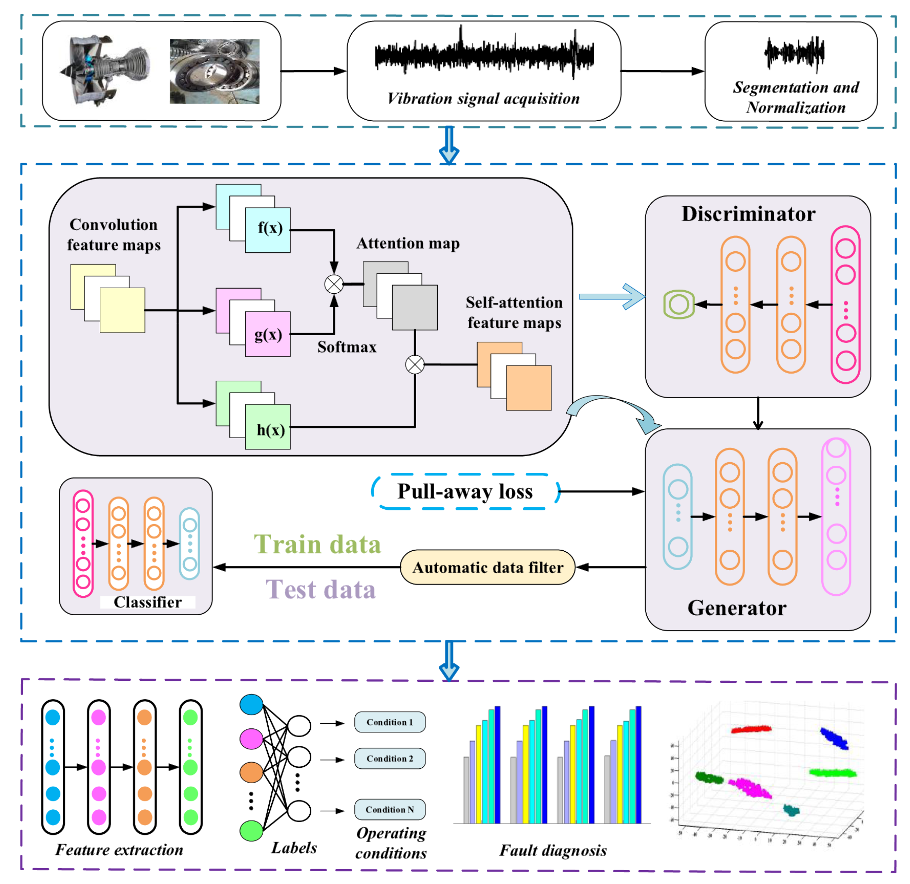
\includegraphics[scale=0.4]{figures/liu.etal_2022.png}
\caption[Roll bearing anomaly methodology]{Methodology for anomaly detection in roll bearing datasets. Taken from \cite{liu.etal_DataSynthesisUsing_2022}.}
\label{fig:liu.etal_2022}
\end{figure}

\begin{description}
    \item[Liu et al. (2022) \cite{liu.etal_DataSynthesisUsing_2022}] propose a deep feature enhanced generative adversarial network to improve fault detection performance in roll bearing imbalanced datasets. New and preexisting methods are introduced to solve mode-collapse during training and enhance the feature learning of the network, which aim to increase the overall detection performance of the architecture. The adopted methodology can be seen in Fig. \ref{fig:liu.etal_2022}.

    A new loss function is designed for the generator with a \textit{pull-away} term. It measures the distance between the generated samples inside a given batch and penalizes the generator if the batch's samples are too similar. As a consequence, this solves the mode-collapse problem during the training phase. A self-attention model is introduced to the discriminator and the generator so they can learn the features of the original vibration signals more deeply. The self-attention feature maps capture local details and global information in every layer of the network.

    During training, the generator synthesizes signals from random noise fed to the discriminator along with an actual signal. The discriminator must then distinguish which one is real and which one is fake. With the proposed mechanisms, the generator must synthesize samples as far as possible to each other to confuse the discriminator. The training phase stops when three criteria are met. These are defined by the \textit{automatic data filter}, which evaluates the accuracy and diversity of the generated samples based on discriminator probability, Kullback-Leibler (KL) divergence and maximum mean discrepancy.  When these criteria surpass a predefined threshold, the training phase is concluded. The fault detection phase uses a classifier trained on the generated data.  

    The quality of synthesised signals was compared with other standard generative models using KL divergence and maximum mean discrepancy of the \textit{automatic data filter}. The proposed method surpassed the others in these metrics. Next, three experiments were set up to evaluate the detection quality of the proposed method. In each experiment, three classifier models were used. In the first, the classifiers learned to detect anomalies from the original signals dataset. In the next, a WGAN-GP architecture was used to generate a more balanced signals dataset. Finally, the three classifiers were trained on data synthesized by the proposed method in the last experiment. This methodology was performed on laboratory and locomotive roll-bearing datasets. Every model trained on the generated data (for both datasets) from the designed solution outperformed the models from the other experiments.

    
\end{description}

% Incomplete
% \begin{description}
%     \item[OD-GAN \cite{oh.etal_OGAN_2019}] is a conditional GAN that uses oversampling to generate samples of the minority class while removing outliers from the majority class. Both the generator $G$ and the discriminator $D$ have the same goals as on the original GAN architecture proposed by Goodfellow et al. \cite{goodfellow.etal_GenerativeAdversarialNets_}. The difference is that in OC-GAN, during training, only the samples of the minority class are considered. The authors define Dissimilarity with the Minority Class score ($DWM_i$), which measures the distance between a sample and the data distribution for the minority class. Samples much further away from the normal distribution have a larger $DWM_i$ and are considered outliers. To detect anomalies, the majority class samples are ordered in accordance with the distance to the minority class. Normal samples lie close to the minority distribution while outliers are recorded when there is a rapid variation in the $DWM_i$ distance.
    
    
%     Data samples that are too close or far away from the minority class are classified as outliers of the majority.
% \end{description}

\begin{description}
    \item[DOPING \cite{lim.etal_DOPINGGenerativeData_2018}] is an adversarial autoencoder that aims to improve the performance of unsupervised anomaly detection by oversampling \textit{infrequent normal samples}. With this, the authors intend to reduce the number of false positives that usually occur on datasets with normal samples close to the classification boundary (close to but not anomalies). 

    In the training phase, the autoencoder receives samples from the entire dataset distribution. The latent vectors generated by the encoder, $E$, from the data samples, $X$, are saved for the next stage, in which only the latent variables $Z$ at the tail-end distribution of the normal data are sampled into a pool of $Z_{edge}$. From this pool, $z_{edge}$ variables are then sampled randomly and interpolated to generate new latent vectors $z_{new}$. In the next stage, de decoder $D$ synthesizes minority samples from the $z_{new}$ latent vectors. Later the synthesized examples can be used in conjunction with the original ones for anomaly detection.

    An isolation forest anomaly detector was used to evaluate the effects of the oversampling method on the detection performance. The authors used three synthesized cluster datasets with outliers, the popular MNIST image dataset, and four real medical record datasets. The results showed that the outlier detection method in conjunction with DOPING achieved better results than the baseline (detection without DOPING). 
\end{description}

\begin{description}
    \item[Bot-GAN \cite{yin.etal_EnhancingFrameworkBotnet_2018}] aims to improve the detection performance of botnets in network-flow data. The architecture is similar to the one from vanilla GAN. However, the authors chose a botnet detection model as a discriminator. Like vanilla GAN, it receives examples from the training dataset and synthesizes ones from the generator. The main difference is that the discriminator classifies each sample as normal (from the training dataset), an anomaly or fake (either synthesized or from the dataset). The generator's objective is to synthesize more samples similar to the ones in the dataset to assist with the training of the detector.

    To test the proposed approach, choose a botnet dataset and perform some preprocessing to normalize the formats of the entries and map the features into vectors. The resulting feature maps are then scaled so that each value falls between [-1,1]. The model was evaluated on precision, accuracy, false positive rate, recall and F1-Score. The results show that it is possible to improve the performance of the classification model by enhancing its training with GANs.
\end{description}

\begin{description}
    \item[Yuan et al. (2020) \cite{yuan.etal_OutageDetectionPartially_2020}] propose employing GANs to learn the normal conditions of smart meter operations to detect power outages in electrical grid zones. In addition, the authors propose circumventing the problems of other models applied to this problem, which are the assumption that every network node is directly observable. The distribution network is subdivided into zones determined by two neighbouring observable nodes (nodes in which the voltage and demand). Each zone has its designated GAN, which learns the time-series data collected by the two nodes. Any deviation from each node's normal measured data distribution will be considered an anomaly.

    The architecture is very similar to the one on vanilla GAN \cite{goodfellow.etal_GenerativeAdversarialNets_}. The generator's objective is to synthesize Time-Windows (frames with recorded sequential events) with events similar to the ones from the assigned zone. Similarly, the discriminator must distinguish between real and fake Time-Windows. At the end of the training phase, both components captured the normality of the data for the given zone.

    In the detection phase, both generator and the discriminator are used. Time-Windows with actual recorded events are fed to the latter, which calculates the Discrimination Loss. Additionally, an inverted mapping of the Time-Window to the latent space is given to the generator, which is tasked with reconstructing it. The weighted sum of the reconstruction error and discriminator loss is used to calculate the Anomaly Score.

    The solution is evaluated on data collected over three years by smart meters on a complex power distribution network. The results proved that the proposed approach could reliably detect power outages in real distribution networks. Finally, numerical comparisons are performed to compare the developed method with a preexisting SMV model to detect power outages. The authors conclude that the developed GAN can achieve better results (in terms of accuracy) with a significantly reduced amount of data.
\end{description}

\begin{description}
    \item[AMBi-GAN \cite{kong.etal_IntegratedGenerativeModel_2023}] is bidirectional LSTM GAN for anomaly detection in industrial multidimensional time-series data. Unlike univariate time series, multivariate time series consists of multiple measurements in a given time step. The authors propose solving the difficulties of other methods in extracting temporal information, feature extraction and lack of large amounts of labelled data.

    The architecture consists of a discriminator and a generator using the same bidirectional LSTM network (AMBi-LSTM). An attention mechanism is also proposed to learn the importance of each time-series element. It calculates a given sample's weight to determine how much it should affect the parameters in the network.

    In the training phase, each sample is extracted using a sliding window that subdivides the whole dataset into equal-length subsequences (each with multiple values for a given time). The generator's goal is to generate windows with the same distribution as the original ones. The discriminator receives real and false samples and must distinguish between them.

    When both components have reached an equilibrium, anomaly detection can be performed. Random samples are extracted from the testing dataset and fed directly to the discriminator. At the same time, the samples suffer from inverted mapping into the latent space, so they can be given to the generator, whose goal is to reconstruct them as well as possible. Next, the \textit{Discriminator Score} is calculated by combining the loss from the discriminator and the reconstruction error from the generator. 

    AMBi-GAN and the other two baselines were evaluated on precision, recall and F1-score on three time-series datasets. The proposed solution outperformed the other baselines on every metric. In addition, several variations of AMBi-GAN were developed, from changing the number of hidden layers of AMBi-LSTM to assess which one performed better on the chosen datasets.
\end{description}

\begin{description}
    \item[TAnoGAN \cite{bashar.nayak_TAnoGANTimeSeries_2020}] was designed to detect anomalies in industrial time-series data with a small number of samples. The model consists of a generator $G$ and a discriminator $D$, with both architectures based on LSTM networks. In the training phase, $G$ learns to generate realistic time-series sequences from a latent space distribution, and $D$ distinguishes fake samples from real ones. The samples consist of small time series sequences extracted from the dataset with a sliding window method. 
    
    In the detection phase, real-time-series samples are mapped to the latent space and then reconstructed by $G$. Anomaly detection is done by evaluating the reconstruction error of the synthesized sample with the original one. Mapping from the original sample to the latent space is done iteratively. First, a random sample $z^i$ from the latent space $z$ is chosen and fed to $G$, which generates a fake sample. The resulting fake data $G(z^i)$ is compared to the original sample $x$ with a point-wise dissimilarity measure $L_R$. Next, the parameters of $z^i$ are updated and thus, in the next iteration, the reconstructed sample will more closely resemble the authentic one. This process is repeated $\Lambda$ times (a predefined parameter). At the end of the inverse mapping, the final $z^i$ is compared to the original sample, and the anomaly score is obtained with the weighted sum of $L_R$ and the discriminator loss $L_D$.

    To deal with the small number of samples in the datasets, the authors varied the number of hidden layers in each architecture. It was observed that discriminators with many hidden layers easily overfitted the data. In contrast, generators with small numbers of hidden layers failed to synthesize realist time series sequences. 

    The solution is evaluated on a large number of time-series datasets along with other unsupervised state-of-the-art anomaly detection methods. The performance (measure in accuracy, recall, F1-score, AUC, and Cohen Kappa Score) demonstrates that TAnoGAN is more suited than other models to detect anomalies in small time-series datasets.
\end{description}

\begin{description}
    \item[MinLGAN \cite{wang.etal_AnomalyDetectionMinimum_2018}] aims to detect outliers by generating both normal and abnormal samples during the training phase. The authors employ minimum likelihood regularisation to the generator, $G$, to produce more abnormal samples and prevent them from converging to the normal distribution of the data. This solution ensures that the performance of the discriminator, $D$, does not deteriorate in the final phases of training as it receives samples from the generator that are increasingly closer to the real distribution of data. The regularization is done by adapting the loss function of the generator with a KL divergence measure. It penalizes the generator when the produced samples are distributed close to the dataset and, thus, prevents the convergence of $G$ with the original data distribution. 

    To deal with the instability of the discriminator in the early phases of training resulting from the data's randomness, the authors propose \textit{Ensemble learning}. Two ensemble methods are presented, which are bagging and boosting. The latter consists of a set of models trained from random subsamples of the training dataset. In contrast, the models are obtained in the former by emphasizing training samples that other models misclassified. The authors independently trained a set of $D$ models in line with this. The outputs of each discriminator (before sigmoid activation) are combined into a single value in two different score functions for anomaly detection (one is scaled to account for the minimum and maximum ranges of the outputs).

    In the experimentation phase, three GANs were created. One baseline MinLGAN and two other models with ensemble learning and the score functions that were defined. All of them were trained along with five other unsupervised anomaly detection approaches on an image and several tabular datasets. Despite providing good results in all datasets, the authors pointed to the difficulty felt in the training phase due to the complexity of the proposed approach.
\end{description}

\begin{description}
    \item[ATTAIN \cite{xu.etal_DigitalTwinbasedAnomaly_2021}] is an architecture that makes use of GANs to detect anomalies in cyber-physical systems (CPS). Unlike other methods, ATTAIN can learn data distribution at runtime without needing static data. This allows it to adapt to previously unseen novel attacks continuously. 

    The solution consists of a Digital Twin Model, a digital replica of a real system, and a Digital Twin Capability; the GAN used for anomaly detection. The first model is built with historical and real-time measurements from sensors and actuators, while the detector only learns from real-time data. The generator's objective is to produce samples from the latent distribution into the original data distribution. The function of the discriminator is to distinguish between normal, and attack samples that come either from real-time or are synthesized by the generator. Therefore, the output of the discriminator consists of four categories. 

    The generator, $G$, is composed of an input layer which encodes discrete values into one-hot vectors; a Graph Convolutional Layer (GCN) that is tasked with learning the independent relationships between sensors and actuators; a pooling layer which collapses the outputs of the previous layers; and an LSTM layer with the function of retaining the temporal features of the data. The discriminator receives both real and generated samples, which are concatenated and suffer a linear transformation. Next, the resulting vector is passed through a \textit{tahn} activation function before being passed to the next layer. The following step calculates a ground truth label for the received fake sample. It is first given to the Digital Twin Model that predicts its state, and later, the hamming distance $d$ between the predicted and real state is obtained to help in the labelling process. The discriminator determines if the sample is real or fake. In the case of the latter the $d$ measure from the previous step is compared to determine if the example is a regular or attack adversarial sample. The loss between the ground truth and the likelihood (obtained by softmax of the output of $D$) is calculated in the final layer.

    The designed model was tested with two other baselines on three intrusion detection datasets. The performance metrics were outlier precision, recall and F1-score. A comparison of all the results shows that using the digital twin model to guide the training of the GAN improved the overall outlier detection capability of the model compared to the other solutions. However, the authors recognize the possible threats to validity as they could not test the solution on a real CPS system. 
\end{description}


\section{Analysis}\label{sec:res_analysis}
In Table \ref{tab:slr_results}, a brief analysis of the SLR results will be carried out to study the effectiveness of the chosen methodology. Aside from the paper name and year, four other categories were identified to compare the evaluated solutions:

\begin{itemize}
    \item \textbf{Training Objective:} this category aims to describe the training approach for a given model. With this, the goal is to compare models that fit the normal data distribution during the training phase and other alternatives. This allows for a straightforward summary of the training approaches that can be adopted to solve the proposed problem.

    \item \textbf{Anomaly Detection:} in this group, the goal is to identify several of the approaches that can be used to detect anomalies. These methods can be relative to calculating an anomaly score or, in some cases, using classifiers to achieve this goal. The possible values for this category include Reconstruction errors, Discriminator Loss (D loss), and Classifiers.

    \item \textbf{Architecture:} this class aims to analyze the different types of architectures defined in each of the papers. These can be "Normal" in the case they use the vanilla architecture of GANs;  "Mixed" when other components like encoders, $E$, classifiers, $C$, feature extractors (FE) and Self-attention devices (SA)\footnote{Module used during the training phase to make the discriminator and generator learn the data features more thoroughly.} are used; and autoencoders (AE).

    \item \textbf{Application:} this last category describes the specific problem that each of the designed models tries to solve (i.e. the scenario to which they are applied). Some models have no direct application and can be used in many types of problems, and because of this, they have no assigned application (N/A)
\end{itemize}



\bgroup
\def\arraystretch{1.5}
\begin{table}
\caption{List of reviewed papers.}
\label{tab:slr_results}
 \begin{adjustwidth}{-1.8cm}{}
\resizebox{0.9\textwidth}{!}{\begin{minipage}{\textwidth}
\centering
\begin{tabular}{cccccc} 
\toprule
\textbf{Paper}         & \textbf{Year} & \textbf{Training Objective}                                                             & \textbf{Anomaly Detection}         & \textbf{Architecture}   & \textbf{Application}                                                        \\ 
\hline
MAD-GAN  \cite{li.etal_MADGANMultivariateAnomaly_2019}     & 2019 & Normal                                                                         & Reconstruction + D loss           & Normal         & Time Series                                                        \\ 
\hline
ALAD \cite{zenati.etal_AdversariallyLearnedAnomaly_2018}         & 2018 & Normal                                                                         & Reconstruction            & Mixed (E)      & N/A                                                                \\ 
\hline
USAD \cite{audibert.etal_USADUnSupervisedAnomaly_2020}         & 2020 & Normal                                                                         & Reconstruction            & AE             & N/A                                                                \\ 
\hline
MO-GAAL \cite{liu.etal_GenerativeAdversarialActive_2020}      & 2020 & \begin{tabular}[c]{@{}c@{}}Outlier Generation \\Division Boundary\end{tabular} & Classifier                & Mixed (C)      & N/A                                                                \\ 
\hline
IGAN-IDS \cite{huang.etal_IGAN_2020}     & 2020 & Outlier Oversampling                                                           & Classifier                & Mixed (FE + C) & Intrusion Detection                                                \\ 
\hline
Jiang et al. \cite{jiang.etal_GANBasedAnomalyDetection_2019}  & 2019 & Normal                                                                         & Reconstruction            & AE             & Time Series                                                        \\ 
\hline
TadGAN \cite{geiger.etal_TadGANTimeSeries_2020}       & 2020 & Normal                                                                         & Reconstruction~ + D loss  & Mixed (E)      & Time Series                                                        \\ 
\hline
adVAE \cite{wang.etal_AdVAESelfadversarialVariational_2020}        & 2020 & Normal                                                                         & Reconstruction            & AE             & N/A                                                                \\ 
\hline
Blance et al. \cite{blance.etal_AdversariallytrainedAutoencodersRobust_2019} & 2019 & Outlier Oversampling                                                           & Classifier                & AE             & High Energy Physics                                                \\ 
\hline
FGPAA \cite{wu.etal_FaultAttentionGenerativeProbabilistic_2020}        & 2020 & Normal                                                                         & Reconstruction            & Mixed (AE)     & Roll Bearing Fault                                                 \\ 
\hline
FGAN \cite{ngo.etal_FenceGANBetter_2019}         & 2019 & \begin{tabular}[c]{@{}c@{}}Normal\\Division Boundary\end{tabular}              & D loss (adapted) & Normal         & N/A                                                                \\ 
\hline
MENSA \cite{siniosoglou.etal_UnifiedDeepLearning_2021}        & 2021 & Normal                                                                         & D (initial layers)        & AE             & Intrusion Detection                                                \\ 
\hline
Liu et al. \cite{liu.etal_DataSynthesisUsing_2022}   & 2022 & Normal                                                                         & Classifier                & Mixed (C + SA) & Roll Bearing Fault                                                 \\ 
\hline
DOPING \cite{lim.etal_DOPINGGenerativeData_2018}       & 2018 & Minority Oversampling                                                          & Classifier/Model          & AE             & \begin{tabular}[c]{@{}c@{}}Performance \\Improvement\end{tabular}  \\ 
\hline
Bot-GAN \cite{yin.etal_EnhancingFrameworkBotnet_2018}      & 2018 & Normal                                                                         & Classifier (D)            & Normal         & Bot Detection                                                      \\ 
\hline
Yuan et al. \cite{yuan.etal_OutageDetectionPartially_2020}   & 2020 & Normal                                                                         & Reconstruction            & Normal         & \begin{tabular}[c]{@{}c@{}}Power Outage \\ Detection\end{tabular}  \\ 
\hline
AMBi-GAN \cite{kong.etal_IntegratedGenerativeModel_2023}      & 2021 & Normal                                                                         & Reconstruction + D loss   & Normal         & Industrial Time Series                                             \\ 
\hline
TAnoGAN \cite{bashar.nayak_TAnoGANTimeSeries_2020}      & 2020 & Normal                                                                         & Reconstruction            & Normal         & Time Series                                                        \\ 
\hline
MinLGAN \cite{wang.etal_AnomalyDetectionMinimum_2018}      & 2018 & All Data                                                                       & D loss                    & Normal         & N/A                                                                \\ 
\hline
ATTAIN \cite{xu.etal_DigitalTwinbasedAnomaly_2021}       & 2021 & Normal                                                                         & D Loss                      & Normal         & Cyber-physical Systems                                             \\
\bottomrule
\end{tabular}
\end{minipage}}
\end{adjustwidth}
\end{table}
\egroup

% \begin{table}[htbp]
% \caption{List of reviewed papers.}
% \label{tab:slr_results}
%  \begin{adjustwidth}{0.5cm}{}
% \resizebox{0.8\textwidth}{!}{\begin{minipage}{\textwidth}
% \begin{tabular}{cccccc} 
% \hline
% Paper                         & Year                      & Training Objective                                                                  & Anomaly Detection                                                    & Architecture                                                    & Application                                                             \\ 
% \hline
% MAD-GAN                       & 2019                      & normal distribution                                                                 & G loss + D loss                                                      & Normal                                                          & Time series                                                             \\ 
% \hline
% ALAD                          & 2018                      & normal distribution                                                                 & Reconstruction                                                       & Mixed (E)                                                       & N/A                                                                     \\ 
% \hline
% USAD                          & 2020                      & normal distriution                                                                  & Reconstruction                                                       & Autoencoder                                                     & N/A                                                                     \\ 
% \hline
% MO-GAAL                       & 2020                      & \begin{tabular}[c]{@{}c@{}}outlier generation\\ division boundary\end{tabular}      & Classifier                                                           & Mixed (C)                                                       & N/A                                                                     \\ 
% \hline
% IGAN-IDS                      & 2020                      & outlier oversampling                                                                & Classifier                                                           & Mixed (FE + C)                                                  & Intrusion detection                                                     \\ 
% \hline
% Jiang et al.                  & 2019                      & normal distribution                                                                 & Reconstruction                                                       & Autoencoder                                                     & Time series                                                             \\ 
% \hline
% TadGAN                        & 2020                      & normal distribution                                                                 & \begin{tabular}[c]{@{}c@{}}Reconstruction \\ and D loss\end{tabular} & Mixed (E)                                                       & Time series                                                             \\ 
% \hline
% adVAE                         & 2020                      & normal distribution                                                                 & Reconstruction                                                       & Autoencoder                                                     & N/A                                                                     \\ 
% \hline
% Blance et al.                 & 2019                      & outlier oversampling                                                                & Classifier                                                           & Autoencoder                                                     & High energy physics                                                     \\ 
% \hline
% FGPAA                         & 2020                      & normal distribution                                                                 & Reconstruction                                                       & \begin{tabular}[c]{@{}c@{}}Autoencoder\\ and G + D\end{tabular} & \begin{tabular}[c]{@{}c@{}}Roll bearing\\ fault detection\end{tabular}  \\ 
% \hline
% FGAN                          & 2019                      & \begin{tabular}[c]{@{}c@{}}normal distribution\\ and division boundary\end{tabular} & \begin{tabular}[c]{@{}c@{}}G loss + D loss \\ (adapted)\end{tabular} & Normal                                                          & N/A                                                                     \\ 
% \hline
% MENSA                         & 2021                      & normal distribution                                                                 & D (initial layers)                                                   & Autoencoder                                                     & Intrusion detection                                                     \\ 
% \hline
% Liu et al.                    & 2022                      & normal distribution                                                                 & Classifier                                                           & \begin{tabular}[c]{@{}c@{}}Mixed\\(C +SA)\end{tabular}          & \begin{tabular}[c]{@{}c@{}}Roll bearing\\fault detection\end{tabular}   \\ 
% \hline
% DOPING                        & 2018                      & \begin{tabular}[c]{@{}c@{}}oversampling\\ normal min.\end{tabular}                  & Classifier/Model                                                     & Autencoder                                                      & \begin{tabular}[c]{@{}c@{}}Performance \\ improvement\end{tabular}      \\ 
% \hline
% Bot-GAN                       & 2018                      & normal distribution                                                                 & Classifier (D)                                                       & Normal                                                          & Bot detection                                                           \\ 
% \hline
% Yuan et al.                   & 2020                      & normal distribution                                                                 & Reconstruction                                                       & Normal                                                          & \begin{tabular}[c]{@{}c@{}}Power outage \\ detection\end{tabular}       \\ 
% \hline
% AMBi-GAN                      & 2021                      & normal distribution                                                                 & \begin{tabular}[c]{@{}c@{}}Reconstruction \\ and D loss\end{tabular} & Normal                                                          & \begin{tabular}[c]{@{}c@{}}Industrial time \\ series\end{tabular}       \\ 
% \hline
% \multicolumn{1}{|c|}{TAnoGAN} & \multicolumn{1}{c|}{2020} & \multicolumn{1}{c|}{normal distribution}                                            & \multicolumn{1}{c|}{Reconstruction}                                  & \multicolumn{1}{c|}{Normal}                                     & \multicolumn{1}{c|}{Time series}                                        \\ 
% \hline
% MinLGAN                       & 2018                      & \begin{tabular}[c]{@{}c@{}}normal and \\ abnormal distributions\end{tabular}        & D                                                                    & Normal                                                          & N/A                                                                     \\ 
% \hline
% ATTAIN                        & 2021                      & normal distribution                                                                 & Loss                                                                 & Normal                                                          & \begin{tabular}[c]{@{}c@{}}Cyber-physical \\ systems\end{tabular}       \\
% \hline
% \end{tabular}
% \end{minipage}}
% \end{adjustwidth}
% \end{table}

\begin{figure}[ht]
\centering
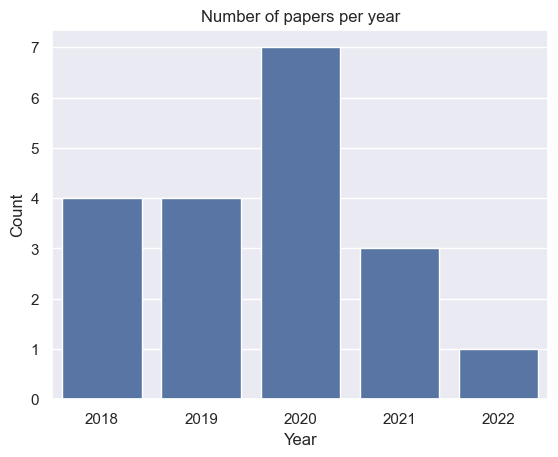
\includegraphics[width=0.5\textwidth]{figures/slr_result_year_paper.png}
\caption{Number of reviewed papers per year. \label{fig:slr_results_year}}
\end{figure}

\begin{figure}[ht]
\centering
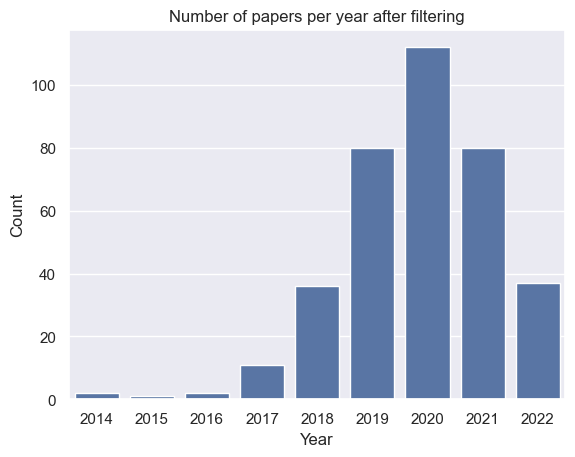
\includegraphics[width=0.5\textwidth]{figures/slr_results_filtering.png}
\caption{Number of reviewed papers after citation filter step (Fig. \ref{fig:slr_pipeline})}
\label{fig:slr_after_filter}
\end{figure}

Fig. \ref{fig:slr_results_year} shows the number of analysed papers per year, and Fig. \ref{fig:slr_after_filter} shows the year distribution of the papers analysed by hand after the application of the citation filter (Fig. \ref{fig:slr_pipeline}). The majority of the papers that were chosen were from 2020. Even after the restrictions applied to the search query, a significant portion of the results is still comprised of GANs for image synthesis.

Further analysis can be done with regard to the search questions defined in sec. \ref{sec:search_questions}. For \textbf{SQ1}, it was shown that several solutions apply GANs or variations in anomaly detection in tabular datasets. Surprisingly, some models worked on image and tabular datasets with the proper adjustments. Additionally, 40\% use either an autoencoder or parts of it to help with anomaly detection in complex data types and 9/20 use some variation of reconstruction errors to determine if a sample is anomalous.

As for \textbf{SQ2}, it was shown that most methods (75\%) learn the normal distribution during the training phase and then detect outliers. 20\% generate outliers that are used to train classifiers for detecting anomalies. Only \cite{wang.etal_AnomalyDetectionMinimum_2018} makes use of both abnormal and normal data distribution in the training phase. This indicates that most GAN-based solutions for anomaly detection can generate realistic data with the same distribution as the original data. However, not all use the discriminator to distinguish between normal and abnormal samples, as they employ classifiers.

\section{Threats to SLR}\label{sec:slr_threats}
The chosen limit for the minimum citations might have been too restrictive, especially for the papers recently published. The adaptation of inclusion criteria I4 (Table \ref{tab:criteria}) to allow for fewer citations in earlier papers was made to try and mitigate this risk. Despite this, the number of analysed papers for 2022 was significantly smaller than the previous years, which introduces the risk that some of the newer published relevant papers might have been overlooked. 

Furthermore, as only one search engine was used for the SLR, there is also the risk that some relevant papers from other platforms were not encountered during this process. 

Another threat may arise due to the terms used to search for relevant papers. After analyzing multiple articles, various synonyms for both GANs and anomalies were collected to reach the most number of papers possible. Despite this, there exists the possibility that some authors didn't use any of these terms to characterize their approach in the title, abstract or keywords of the document. This way, there is a small risk that some relevant papers might have eluded the search query.

Similarly, by prohibiting documents that referenced images, or anything other than tabular data, some relevant papers might have been excluded. This can occur, for instance, in architectures that were firstly designed for image anomaly detection but were also suited for tabular datasets.

\section{Summary}\label{sec:summary}
This chapter explained the methodology used to aggregate the papers relevant to the problem in question. First, a set of search questions were defined (sec. \ref{sec:search_questions} followed by the respective query (sec. \ref{sec:search_queries}) that was used on Scopus. The selection criteria and the processing pipeline were delined in Section \ref{sec:inclusion_exclusion}. A summary of each of the selected papers is provided in Section \ref{sec:stoa_results}. Next, a categorization and summary of the entire process are performed in Section \ref{sec:res_analysis}, followed by the threats to the SLR process (sec. \ref{sec:slr_threats}).


% TODO rever anomaly method para USAD
% TODO rever blance et al.



